% detailed  presentation of a model, including justifications for design decisions

Figure \ref{fig:MultilevelArchitecture} shows the overview of the multivel architecture designed to capture the two use cases described in the Process Challenge.

% Expliquer que le use case XSure ne nécessitait pas l'extension de metamodèle requise pour le usecase Acme Software Developement Process

\subsection{Base metamodel for the Process Challenge}

\begin{figure*}
 \centering
    % 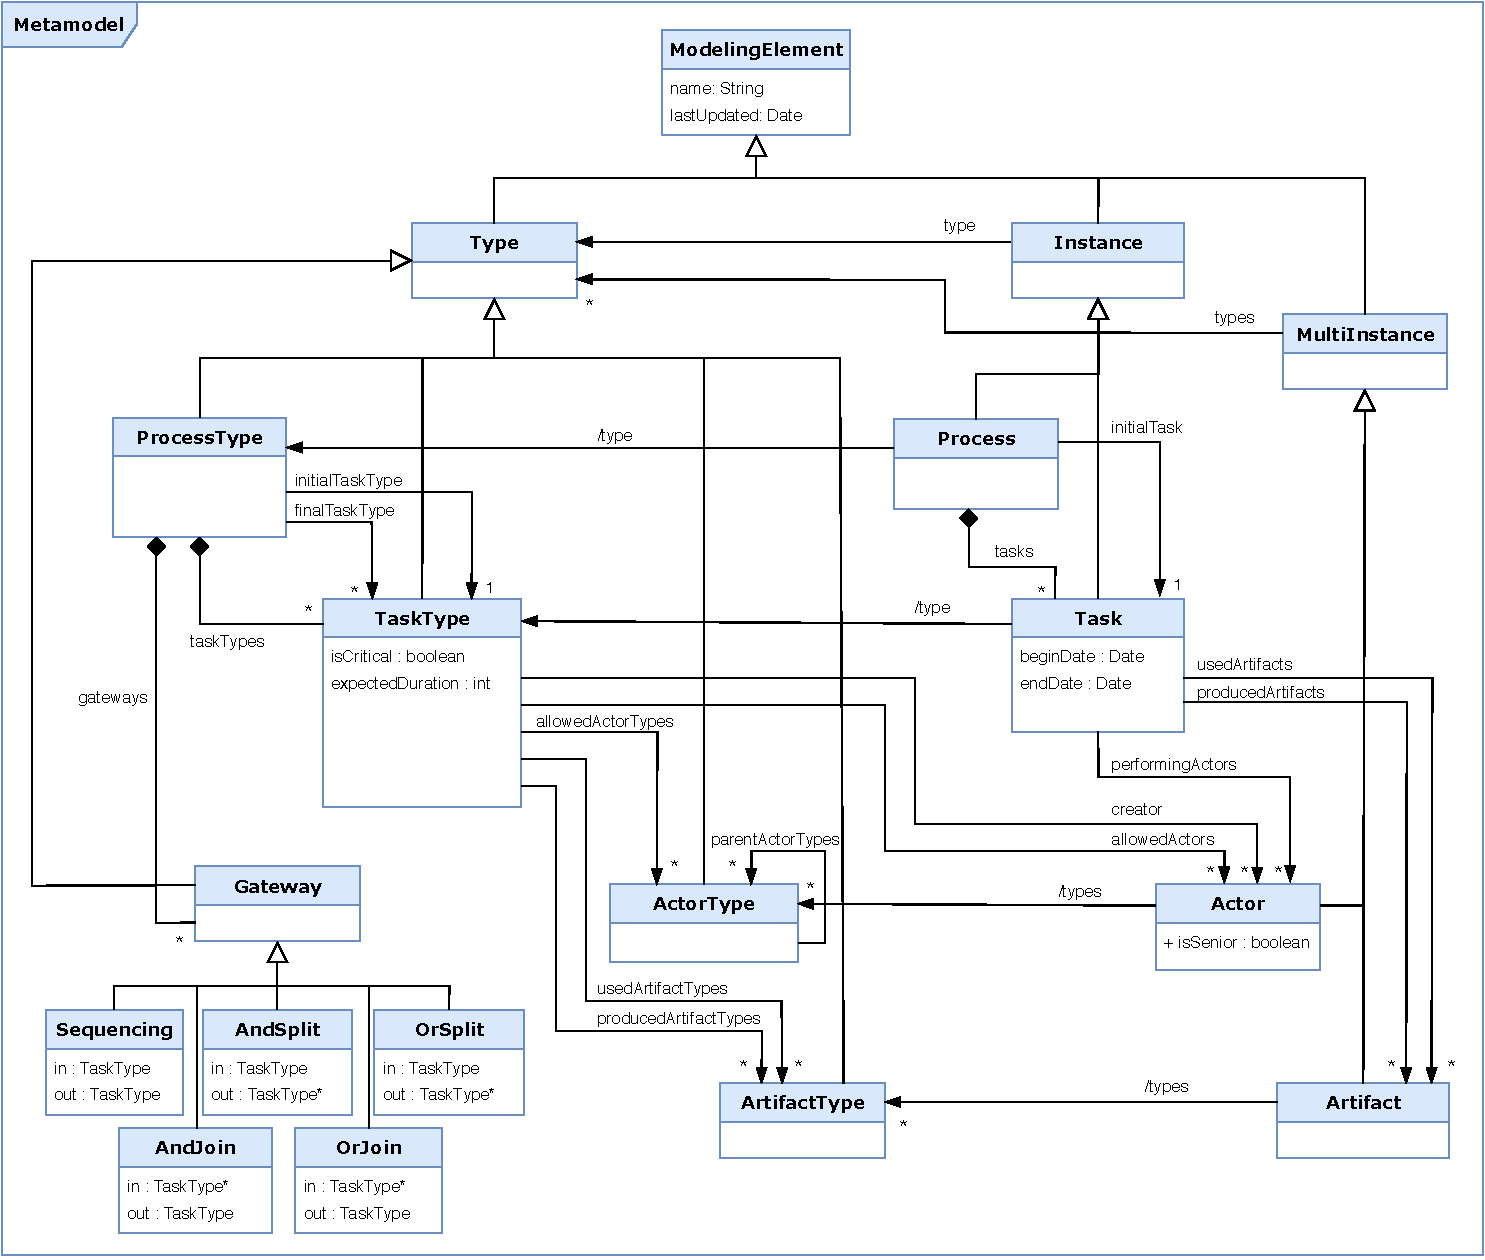
\includegraphics[width=1.0 \columnwidth]{Figures/Metamodel.pdf}
    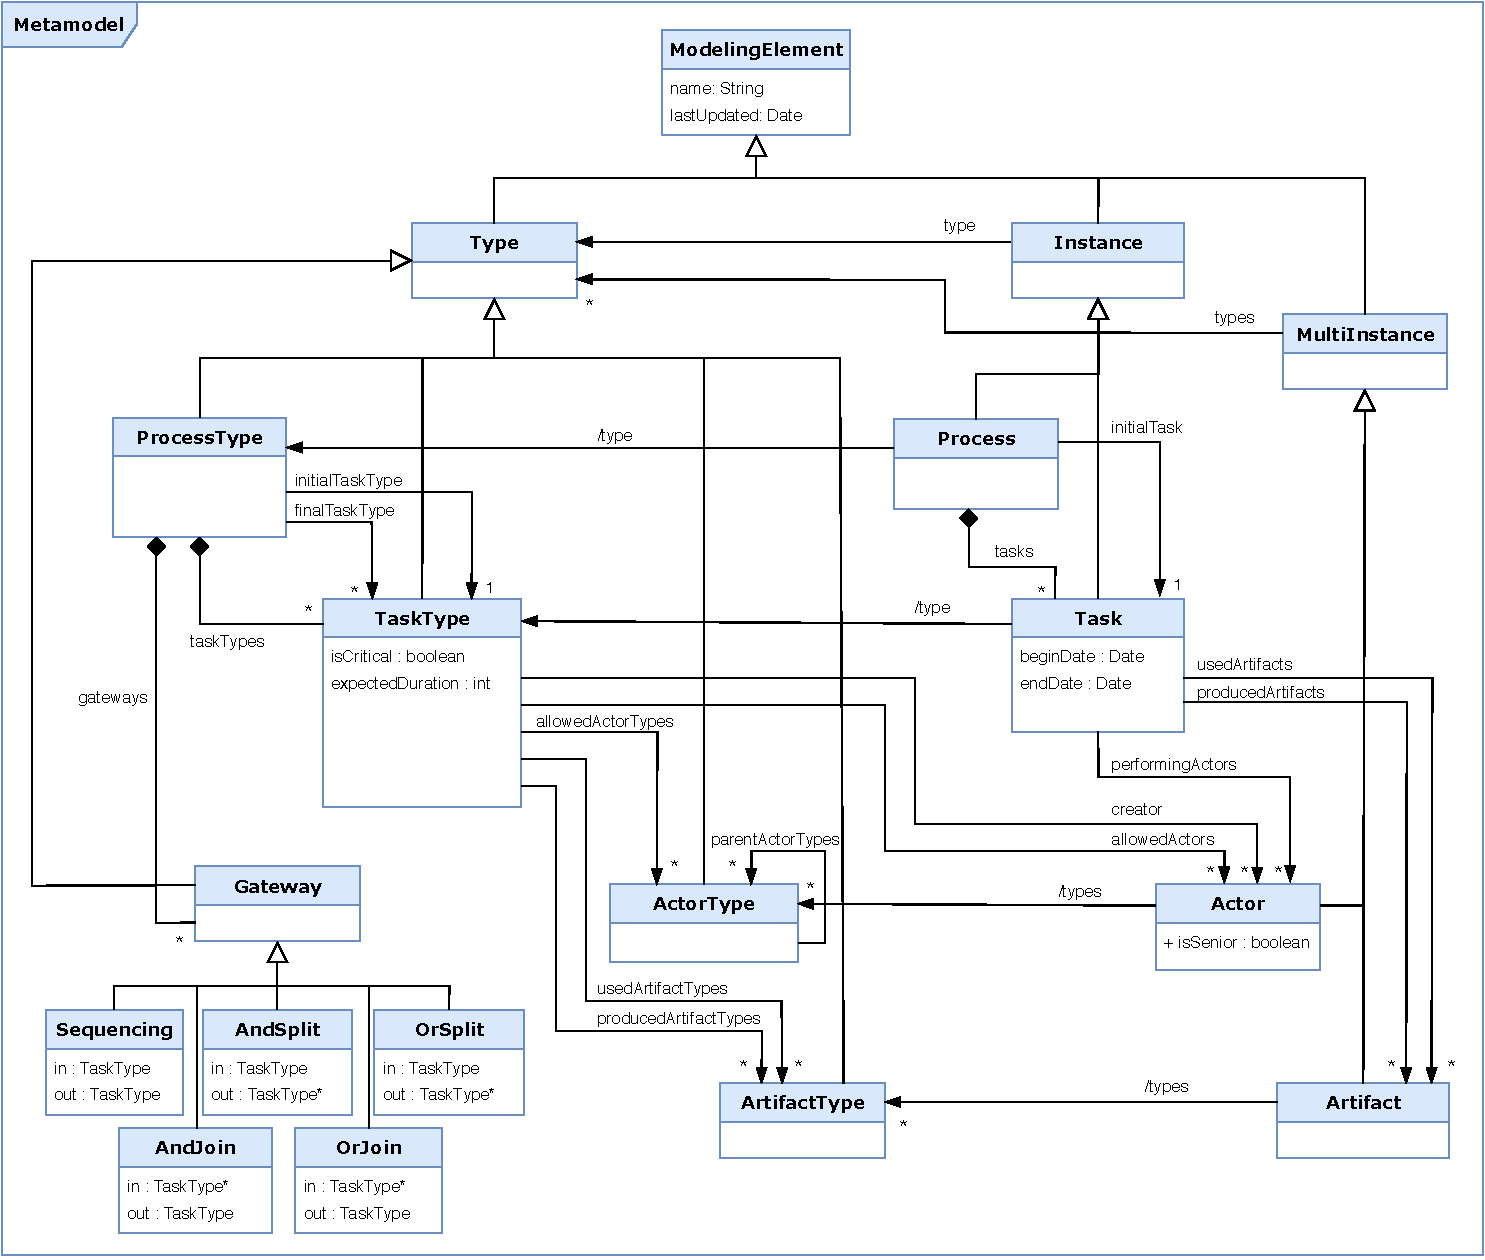
\includegraphics[width=1.0 \textwidth]{Figures/Metamodel.pdf}
    \caption{Process management base metamodel}
    \label{fig:BaseMetamodel}
\end{figure*}

\subsection{The XSure insurance domain}

We will illustrate the base metamodel presented in this section with XSure insurance domain use case, whose a partial description was provided in the challenge description. Note that the capture of the requirements P1 to P19 in the context of XSure insurance domain are straightforward implementable while instantiating base metamodel presented in figure \ref{fig:BaseMetamodel}.

The use case presented in this section is straightforward implementable while instantiating base metamodel presented in figure \ref{fig:BaseMetamodel}.

% Passer rapidement sur ce cas pour illustrer le metamodèle décrit plus haut

% We will illustrate the approach...

\subsection{The Acme software development process}

\subsection{Openflexo tooling}

% Expliquer l'outillage construit et comment il marche


